
\subsection{Programming languages and Libraries}

C\# was selected for this project because of its widespread popularity in
enterprise applications and its capability to operate across various operating
systems following the release of .NET Core. This feature significantly enhances
deployment flexibility, allowing the application to be utilized in diverse
environments. 

Additionally, we have incorporated ASP.NET Core specifically version 8 into our
technology stack. By leveraging ASP.NET Core, we benefit from a robust,
well-supported framework that facilitates the development of scalable and secure
web applications. It seamlessly integrates with C\#, enabling us to utilize a
consistent programming environment while also exploiting features such as
dependency injection, a vast ecosystem of middleware, and a strong configuration
system that is suited to modern web applications.

ASP.NET Core 8 brings forward improvements in areas such as minimized startup
times, reduced memory footprint, and enhanced security features, making it an
ideal choice for developing scalable and secure web applications. The choice
also underscores our commitment to developing applications that are both
efficient and future-proof, ensuring that they perform optimally on both Windows
and non-Windows platforms. This alignment with .NET Core’s cross-platform
capabilities ensures that our project remains versatile and adaptable to the
evolving technological landscape.

Optionally, we have integrated the Nuxt framework into our technology stack.
Nuxt is a progressive Vue framework that is used for building more robust and
versatile web applications. It simplifies the development process by handling
various aspects of the web infrastructure, such as server-side rendering, static
site generation, and automatic code splitting. This inclusion enriches our
application's interactivity and user experience, providing a seamless and
dynamic interface for users.

\subsection{Command Query Responsibility Segregation}

The Command Query Responsibility Segregation (CQRS) is an architectural pattern
that distinctively separates the tasks of reading data (queries) and writing
data (commands) within a software application. This separation splits
responsibilities into two main components:

\begin{itemize}
\item \textbf{Command Side}: This component manages operations that modify the
system's state. It handles incoming commands from clients or external systems,
conducts validations, and updates the data store accordingly. This side is
essential for maintaining the integrity and accuracy of data modifications
within the application.
\item \textbf{Query Side}: Dedicated to data retrieval, this component processes
all read requests. It fetches data from the appropriate sources, ensuring that
the information provided is accurate and reflects the current state of the data
store.
\end{itemize}

Key advantages of employing the CQRS pattern are:

\begin{itemize}
\item \textbf{Scalability}: CQRS allows for the independent scaling of the read
and write components based on their respective workloads, which can
significantly enhance system performance.
\item \textbf{Flexibility}: With the separation of concerns, different storage
and optimization strategies can be applied to the reading and writing processes.
This flexibility enables the use of the most appropriate tools for each
function, optimizing efficiency.
\item \textbf{Event-Driven Architecture Compatibility}: The use of CQRS often
complements event-driven architectures, where changes in the system's state are
captured and managed as events. This compatibility ensures that the architecture
is dynamic and responsive to changes in business requirements.
\end{itemize}

\subsection{Project Structure}

\begin{figure}[H]
  \centering
  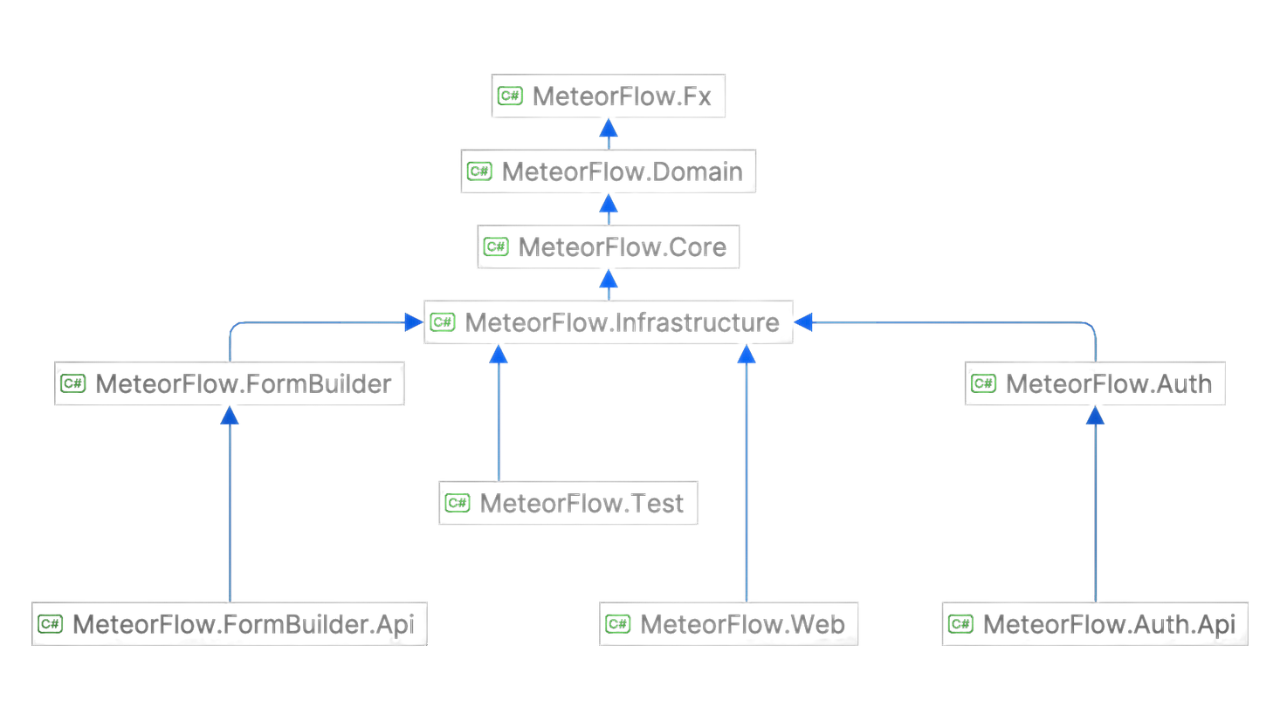
\includegraphics[width=\linewidth]{Images/ProjectDir.png}
  \caption{Project Structure}
\end{figure}

MeteorFlow is depicted as a modular framework comprising several interdependent
components. Each library or module serves a distinct function, collectively
supporting a robust and scalable application infrastructure. This section will
delineate the roles and relationships of these components.

MeteorFlow.Fx enriches the application by introducing additional functionalities
or user interface enhancements. These features, while not central to the primary
business logic, significantly augment the application’s overall capabilities,
providing enriched user experiences and functional extensions.

MeteorFlow.Domain is tailored to articulate the business domain, encapsulating
entities and rules essential to the application's domain logic. Its reliance on
the Core module underscores the latter’s foundational role within the
architecture, affirming its influence over the domain-specific functionalities.

At the heart of the architecture, MeteorFlow.Core embodies the fundamental
business logic and operations critical to the application. Its pivotal role is
underscored by its influence on all peripheral modules, which depend on the Core
for their foundational functionalities.

MeteorFlow.Infrastructure functions as the backbone for data access and manages
cross-cutting concerns such as logging and caching. This module is crucial for
the operational management of the application, interfacing seamlessly with the
Core module to apply essential functionalities across various infrastructural
tasks.

Built upon the MeteorFlow.Infrastructure, the Auth module specializes in
security and authentication processes, managing user verification and credential
handling. The module provides APIs to enable external access to their functionalities and
seamlessly integrate with other systems and applications. Other modules
currently or in the near future follow the same structure above to provide
additional functionalities.

MeteorFlow.Web, primarily tasked with managing the application’s API gateway,
interacts with all other modules within MeteorFlow to ensure robust web
operations and effective resource management. Its role is crucial in maintaining
the integrity and performance of web-based services, underpinning the system's
interaction with users and external systems.


